\documentclass[11pt,a4paper]{article}
\usepackage[dvipsnames]{xcolor}
\usepackage{amsmath,tabularx,geometry,graphicx,multirow,tikz,listings,xfrac}

\usetikzlibrary{positioning}
\newdimen\nodeDist
\nodeDist=35mm
\geometry{a4paper, left=20mm, top=20mm}
\graphicspath{{../imgs/}}
\newcommand\sbullet[1][.5]{\mathbin{\vcenter{\hbox{\scalebox{#1}{$\bullet$}}}}}
\newcommand{\circo}{~\raisebox{1pt}{\tikz \draw[line width=0.5pt] circle(1.1pt);}~}

\title{Aprendizagem 2021/22 Homework III - Group 66}
\author{João Cardoso, 99251. José João Ferreira, 99259}

\begin{document}

\color{darkgray}
\hspace{-8.25mm}
\renewcommand\tabularxcolumn[1]{m{#1}}
\begin{tabularx}{1.09\textwidth} {>{\raggedright\arraybackslash}X >{\centering\arraybackslash}X >{\raggedleft\arraybackslash}X}
  
\includegraphics[scale=0.2]{tecnico.pdf} &
  \textbf{Aprendizagem 2022/23} \par \textbf{Homework III - Group 66} &
  João Cardoso, 99251 \par José João Ferreira, 99259
\end{tabularx}
\renewcommand\tabularxcolumn[1]{p{#1}}
\color{black}

\begin{center}
\textbf{I. Pen-and-paper}
\end{center}

% PROBLEM 1
\begin{flushleft}
\textbf{1)}
\small
\begin{tabularx}{1.09\textwidth}{>{\hsize=.65\hsize}X X X}
  \begin{tabular}{c|c|c}
    $j$ & $x_j$ & $z_j$ \\ \hline
    1   & 0.8   & 24    \\
    2   & 1     & 20    \\
    3   & 1.2   & 10    \\
    4   & 1.4   & 13    \\
    5   & 1.6   & 12   
  \end{tabular}
  &
  \vspace{-23.5mm}{\begin{flalign*}
    (\hat{z}, w) & = \sum_{j=0}^3 w_j \phi_j(x) &&\\
    & = w_0 + w_1x + w_2x^2 + w_3x^3 &&\\
  \end{flalign*}
  \vspace{-15mm}\begin{flalign*}
    Xw = Z & \Leftrightarrow X^TXw = X^TZ &&\\
    & \Leftrightarrow (X^TX)^{-1}X^TXw = (X^TX)^{-1}X^TZ &&\\
    & \Leftrightarrow w = (X^TX)^{-1}X^TZ &&\\
  \end{flalign*}
  \vspace{-15mm}\begin{flalign*}
    & \text{Ridge regression:} \quad w = (X^TX + \lambda I)^{-1}X^TZ &&\\
  \end{flalign*}}
  &
  \vspace{-20mm}{\begin{flalign*}
    && X = \begin{pmatrix}
      1 & 0.8 & 0.8^2 & 0.8^3 \\
      1 & 1 & 1^2 & 1^3 \\
      1 & 1.2 & 1.2^2 & 1.2^3 \\
      1 & 1.4 & 1.4^2 & 1.4^3 \\
      1 & 1.6 & 1.6^2 & 1.6^3
    \end{pmatrix}
  \end{flalign*}} \par \hspace{4.25mm}
  $ \lambda = 2 $
\end{tabularx}

\vspace{-12.5mm}\begin{flalign*}
  & X^TX = \begin{pmatrix}
    1 & 1 & 1 & 1 & 1 \\
    0.8 & 1 & 1.2 & 1.4 & 1.6 \\
    0.64 & 1 & 1.44 & 1.96 & 2.56 \\
    0.512 & 1 & 1.728 & 2.744 & 4.096
  \end{pmatrix}
  \begin{pmatrix}
    1 & 0.8 & 0.64 & 0.512 \\
    1 & 1 & 1 & 1 \\
    1 & 1.2 & 1.44 & 1.728 \\
    1 & 1.4 & 1.96 & 2.744 \\
    1 & 1.6 & 2.56 & 4.096
  \end{pmatrix} =
  \begin{pmatrix}
    5 & 6 & 7.6 & 10.08 \\
    6 & 7.6 & 10.08 & 13.8784 \\
    7.6 & 10.08 & 13.8784 & 19.68 \\
    10.08 & 13.8784 & 19.68 & 28.5549
  \end{pmatrix} &&\\
\end{flalign*}

\vspace{-12.5mm}\begin{flalign*}
  & X^TX + \lambda I = \begin{pmatrix}
    5 & 6 & 7.6 & 10.08 \\
    6 & 7.6 & 10.08 & 13.8784 \\
    7.6 & 10.08 & 13.8784 & 19.68 \\
    10.08 & 13.8784 & 19.68 & 28.5549
  \end{pmatrix} +
  \begin{pmatrix}
    2 & 0 & 0 & 0 \\
    0 & 2 & 0 & 0 \\
    0 & 0 & 2 & 0 \\
    0 & 0 & 0 & 2 \\
  \end{pmatrix} =
  \begin{pmatrix}
    7 & 6 & 7.6 & 10.08 \\
    6 & 9.6 & 10.08 & 13.8784 \\
    7.6 & 10.08 & 15.8784 & 19.68 \\
    10.08 & 13.8784 & 19.68 & 30.5549
  \end{pmatrix} &&\\
\end{flalign*}

\vspace{-12.5mm}\begin{flalign*}
  w &= \begin{pmatrix}
    7 & 6 & 7.6 & 10.08 \\
    6 & 9.6 & 10.08 & 13.8784 \\
    7.6 & 10.08 & 15.8784 & 19.68 \\
    10.08 & 13.8784 & 19.68 & 30.5549
  \end{pmatrix}^{-1}
  \begin{pmatrix}
    1 & 1 & 1 & 1 & 1 \\
    0.8 & 1 & 1.2 & 1.4 & 1.6 \\
    0.64 & 1 & 1.44 & 1.96 & 2.56 \\
    0.512 & 1 & 1.728 & 2.744 & 4.096
  \end{pmatrix}
  \begin{pmatrix}
    24 \\ 20 \\ 10 \\ 13 \\ 12
  \end{pmatrix} &&\\
  &= \begin{pmatrix}
    0.341688 & -0.121426 & -0.074902 & -0.009325 \\
    -0.121426 & 0.389208 & -0.096677 & -0.074456 \\
    -0.074902 & -0.096677 & 0.372577 & -0.171350 \\
    -0.009325 & -0.074456 & -0.171350 & 0.179987
  \end{pmatrix}
  \begin{pmatrix}
    79 \\ 88.6 \\ 105.96 \\ 134.392
  \end{pmatrix} =
  \textcolor{ForestGreen}{\begin{pmatrix}
    7.045076 \\ 4.640926 \\ 1.967336 \\ -1.300877
  \end{pmatrix}} &&\\
\end{flalign*}
\end{flushleft}
\normalsize

% PROBLEM 2
\begin{flushleft}
\vspace{-2mm}
\textbf{2)}
\small
\vspace{-2mm}\begin{flalign*}
  & \hat{z} = w_0 + w_1x + w_2x^2 + w_3x^3 \quad \Longrightarrow \quad \hat{Z} = Xw &&\\[2mm]
  & \hat{Z} = \begin{pmatrix}
    1 & 0.8 & 0.64 & 0.512 \\
    1 & 1 & 1 & 1 \\
    1 & 1.2 & 1.44 & 1.728 \\
    1 & 1.4 & 1.96 & 2.744 \\
    1 & 1.6 & 2.56 & 4.096
  \end{pmatrix}
  \begin{pmatrix}
    7.045076 \\ 4.640926 \\ 1.967336 \\ -1.300877
  \end{pmatrix} =
  \begin{pmatrix}
    11.350863 \\ 12.352461 \\ 13.199236 \\ 13.828744 \\ 14.178546
  \end{pmatrix} &&\\[2mm]
  & Z^T = \begin{pmatrix} 24 & 20 & 10 & 13 & 12 \end{pmatrix}, \quad \hat{Z}^T = \begin{pmatrix} 11.35086 & 12.35246 & 13.19924 & 13.82874 & 14.17855 \end{pmatrix} &&\\
  & \sum_{i = 1}^n (z_i - \hat{z}_i)^2 = (24 - 11.35086)^2 + (20 - 12.35246)^2 + (10 - 13.19924)^2 + (13 - 13.82874)^2 + (12 - 14.17855)^2 &&\\[-2mm]
  & RMSE(z, \hat{z}) = \sqrt{\frac{1}{n}\sum_{i = 1}^n (z_i - \hat{z}_i)^2} \quad \Longrightarrow \quad RMSE(z, \hat{z}) = \sqrt{\frac{1}{5} \times 234.153637} \approx \textcolor{ForestGreen}{6.843298} &&\\
\end{flalign*}
\end{flushleft}
\normalsize

\pagebreak
\color{darkgray}
\hspace{-8.25mm}
\renewcommand\tabularxcolumn[1]{m{#1}}
\begin{tabularx}{1.09\textwidth} {>{\raggedright\arraybackslash}X >{\centering\arraybackslash}X >{\raggedleft\arraybackslash}X}
  
\includegraphics[scale=0.2]{tecnico.pdf} &
  \textbf{Aprendizagem 2022/23} \par \textbf{Homework III - Group 66} &
  João Cardoso, 99251 \par José João Ferreira, 99259
\end{tabularx}
\renewcommand\tabularxcolumn[1]{p{#1}}
\color{black}

\begin{center}
\textbf{}
\end{center}

% PROBLEM 3
\begin{flushleft}
\textbf{3)}
\par $\sbullet$ \underline{1st step: forward propagation} \par
\small
\begin{tabularx}{1.09\textwidth}{X X}
  \vspace{1.5mm} % Formulas
  $ f(x) = e^{0.1(x)} \quad\quad f'(x) = 0.1e^{0.1(x)} $ \par \vspace{1mm}
  $ w^{[1]} = \begin{pmatrix} 1 \\ 1 \end{pmatrix} \quad b^{[1]} = \begin{pmatrix} 1 \\ 1 \end{pmatrix} \quad w^{[2]} = \begin{pmatrix} 1 & 1 \end{pmatrix} \quad b^{[2]} = \begin{pmatrix} 1 \end{pmatrix} $ \par \vspace{1mm}
  $ a^{[1]} = w^{[1]}x + b^{[1]} $ \par \vspace{1mm}
  $ h^{[1]} = f(a^{[1]}) $ \par \vspace{1mm}
  $ a^{[2]} = w^{[2]}h^{[1]} + b^{[2]} $ \par \vspace{1mm}
  $ h^{[2]} = f(a^{[2]}) $ \par \vspace{1mm}
  & % X_1
  $ \boxed{x_1 = 0.8} \quad z_1 = 24 $ \par \vspace{1mm}
  $ a^{[1]} = \begin{pmatrix} 1 \\ 1 \end{pmatrix} \begin{pmatrix} 0.8 \end{pmatrix} + \begin{pmatrix} 1 \\ 1 \end{pmatrix} = \begin{pmatrix} 1.8 \\ 1.8 \end{pmatrix} $ \par \vspace{1mm}
  $ h^{[1]} = f \begin{pmatrix} 1.8 \\ 1.8 \end{pmatrix} = \begin{pmatrix} e^{0.1(1.8)} \\ e^{0.1(1.8)} \end{pmatrix} \approx \begin{pmatrix} 1.197217 \\ 1.197217 \end{pmatrix} $ \par \vspace{1mm}
  $ a^{[2]} = \begin{pmatrix} 1 & 1 \end{pmatrix} \begin{pmatrix} 1.197217 \\ 1.197217 \end{pmatrix} + \begin{pmatrix} 1 \end{pmatrix} = 3.394435 $ \par \vspace{1mm}
  $ h^{[2]} = f \begin{pmatrix} 3.394435 \end{pmatrix} = e^{0.1(3.394435)} \approx 1.404166 $ \par \vspace{1mm}
\end{tabularx}
\begin{tabularx}{1.09\textwidth}{X X}
  % X_2
  $ \boxed{x_2 = 1} \quad z_2 = 20 $ \par \vspace{1mm}
  $ a^{[1]} = \begin{pmatrix} 1 \\ 1 \end{pmatrix} \begin{pmatrix} 1 \end{pmatrix} + \begin{pmatrix} 1 \\ 1 \end{pmatrix} = \begin{pmatrix} 2 \\ 2 \end{pmatrix} $ \par \vspace{1mm}
  $ h^{[1]} = f \begin{pmatrix} 2 \\ 2 \end{pmatrix} = \begin{pmatrix} e^{0.1(2)} \\ e^{0.1(2)} \end{pmatrix} \approx \begin{pmatrix} 1.221402 \\ 1.221402 \end{pmatrix} $ \par \vspace{1mm}
  $ a^{[2]} = \begin{pmatrix} 1 & 1 \end{pmatrix} \begin{pmatrix} 1.221402 \\ 1.221402 \end{pmatrix} + \begin{pmatrix} 1 \end{pmatrix} = 3.442806 $ \par \vspace{1mm}
  $ h^{[2]} = f \begin{pmatrix} 3.442806 \end{pmatrix} = e^{0.1(3.442806)} \approx 1.410974 $ \par \vspace{1mm}
  & % X_3
  $ \boxed{x_3 = 1.2} \quad z_3 = 10 $ \par \vspace{1mm}
  $ a^{[1]} = \begin{pmatrix} 1 \\ 1 \end{pmatrix} \begin{pmatrix} 1.2 \end{pmatrix} + \begin{pmatrix} 1 \\ 1 \end{pmatrix} = \begin{pmatrix} 2.2 \\ 2.2 \end{pmatrix} $ \par \vspace{1mm}
  $ h^{[1]} = f \begin{pmatrix} 2.2 \\ 2.2 \end{pmatrix} = \begin{pmatrix} e^{0.1(2.2)} \\ e^{0.1(2.2)} \end{pmatrix} \approx \begin{pmatrix} 1.246077 \\ 1.246077 \end{pmatrix} $ \par \vspace{1mm}
  $ a^{[2]} = \begin{pmatrix} 1 & 1 \end{pmatrix} \begin{pmatrix} 1.246077 \\ 1.246077 \end{pmatrix} + \begin{pmatrix} 1 \end{pmatrix} = 3.492153 $ \par \vspace{1mm}
  $ h^{[2]} = f \begin{pmatrix} 3.492153 \end{pmatrix} = e^{0.1(3.492153)} \approx 1.417955 $ \par \vspace{1mm}
\end{tabularx}

\normalsize $\sbullet$ \underline{2nd step: back propagation} \par \small
\begin{align*}
  E_k = \frac{1}{2}(h^{[2]}_k - z_k)^2 \quad\quad\quad
  h^{[L]} = f(a^{[L]}) \quad\quad\quad
  a^{[L]} = w^{[L]}h^{[L-1]} + b^{[L]}
\end{align*}
\vspace{-7.5mm}
\begin{align*}
  \frac{\partial E_k}{\partial h^{[2]}} = h^{[2]}_k - z_k \quad\quad\quad
  \frac{\partial h^{[L]}}{\partial a^{[L]}} = f'(a^{[L]}) \quad\quad\quad
  \frac{\partial a^{[L]}}{\partial w^{[L]}} = h^{[L-1]} \quad\quad\quad
  \frac{\partial a^{[L]}}{\partial h^{[L-1]}} = w^{[L]} \quad\quad\quad
  \frac{\partial a^{[L]}}{\partial b^{[L]}} = 1
\end{align*}
% dE/dw^[2]
\begin{flalign*}
  & \frac{\partial E_k}{\partial w^{[2]}} = \frac{\partial E_k}{\partial h^{[2]}_k} \frac{\partial h^{[2]}_k}{\partial a^{[2]}_k} \frac{\partial a^{[2]}_k}{\partial w^{[2]}} = (h^{[2]}_k - z_k) \cdot f'(a^{[2]}_k) \cdot h_k^{[1]^T} &&\\[1mm]
  & x_1: \quad \frac{\partial E_1}{\partial w^{[2]}} = (1.404166 - 24) \cdot (0.1 \times 1.404166) \cdot \begin{pmatrix} 1.197217 & 1.197217 \end{pmatrix} \approx \begin{pmatrix} -3.798566 & -3.798566 \end{pmatrix} &&\\
  & x_2: \quad \frac{\partial E_2}{\partial w^{[2]}} = (1.410974 - 20) \cdot (0.1 \times 1.410974) \cdot \begin{pmatrix} 1.221402 & 1.221402 \end{pmatrix} \approx \begin{pmatrix} -3.203570 & -3.203570 \end{pmatrix} &&\\
  & x_3: \quad \frac{\partial E_3}{\partial w^{[2]}} = (1.417955 - 10) \cdot (0.1 \times 1.417955) \cdot \begin{pmatrix} 1.246077 & 1.246077 \end{pmatrix} \approx \begin{pmatrix} -1.516345 & -1.516345 \end{pmatrix} &&\\
  & \frac{\partial E}{\partial w^{[2]}} = \sum_{k = 1}^{3}\frac{\partial E_k}{\partial w^{[2]}} = \begin{pmatrix} -8.518481 & -8.518481 \end{pmatrix} &&\\
  & \textcolor{ForestGreen}{w^{[2]}_{new}} = w^{[2]}_{old} - \eta \frac{\partial E}{\partial w^{[2]}} = \begin{pmatrix} 1 & 1 \end{pmatrix} - 0.1 \begin{pmatrix} -8.518481 & -8.518481 \end{pmatrix} \approx \textcolor{ForestGreen}{\begin{pmatrix} 1.851848 & 1.851848 \end{pmatrix}} &&\\
\end{flalign*}
\end{flushleft}
\normalsize

\pagebreak
\color{darkgray}
\hspace{-8.25mm}
\renewcommand\tabularxcolumn[1]{m{#1}}
\begin{tabularx}{1.09\textwidth} {>{\raggedright\arraybackslash}X >{\centering\arraybackslash}X >{\raggedleft\arraybackslash}X}
  
\includegraphics[scale=0.2]{tecnico.pdf} &
  \textbf{Aprendizagem 2022/23} \par \textbf{Homework III - Group 66} &
  João Cardoso, 99251 \par José João Ferreira, 99259
\end{tabularx}
\renewcommand\tabularxcolumn[1]{p{#1}}
\color{black}

\begin{center}
\textbf{}
\end{center}

\begin{flushleft}\small
% dE/db^[2]
\begin{flalign*}
  & \frac{\partial E_k}{\partial b^{[2]}} = \frac{\partial E_k}{\partial h^{[2]}_k} \frac{\partial h^{[2]}_k}{\partial a^{[2]}_k} \frac{\partial a^{[2]}_k}{\partial b^{[2]}} = (h^{[2]}_k - z_k) \cdot f'(a^{[2]}_k) \cdot 1 &&\\[1mm]
  & x_1: \quad \frac{\partial E_1}{\partial b^{[2]}} = (1.404166 - 24) \cdot (0.1 \times 1.404166) \approx \begin{pmatrix} -3.172830 \end{pmatrix} &&\\
  & x_2: \quad \frac{\partial E_2}{\partial b^{[2]}} = (1.410974 - 20) \cdot (0.1 \times 1.410974) \approx \begin{pmatrix} -2.622863 \end{pmatrix} &&\\
  & x_3: \quad \frac{\partial E_3}{\partial b^{[2]}} = (1.417955 - 10) \cdot (0.1 \times 1.417955) \approx \begin{pmatrix} -1.216895 \end{pmatrix} &&\\
  & \frac{\partial E}{\partial b^{[2]}} = \sum_{k = 1}^{3}\frac{\partial E_k}{\partial b^{[2]}} = \begin{pmatrix} -7.012588 \end{pmatrix} &&\\
  & \textcolor{ForestGreen}{b^{[2]}_{new}} = b^{[2]}_{old} - \eta \frac{\partial E}{\partial b^{[2]}} = \begin{pmatrix} 1 \end{pmatrix} - 0.1 \begin{pmatrix} -7.012588 \end{pmatrix} \approx \textcolor{ForestGreen}{\begin{pmatrix} 1.701259 \end{pmatrix}} &&\\
\end{flalign*}
% dE/dw^[1]
\vspace{-3.75mm}\begin{flalign*}
  & \frac{\partial E_k}{\partial w^{[1]}} = \frac{\partial E_k}{\partial h^{[2]}_k} \frac{\partial h^{[2]}_k}{\partial a^{[2]}_k} \frac{\partial a^{[2]}_k}{\partial h^{[1]}_k} \frac{\partial h^{[1]}_k}{\partial a^{[1]}_k} \frac{\partial a^{[1]}_k}{\partial w^{[1]}} = w^{[2]^T} \cdot (h^{[2]}_k - z_k) \cdot f'(a^{[2]}_k) \cdot f'(a^{[1]}_k) \cdot x^T_k &&\\[1mm]
  & x_1: \quad \frac{\partial E_1}{\partial w^{[1]}} = \begin{pmatrix} 1 \\ 1 \end{pmatrix} \cdot (-3.172830) \circo \begin{pmatrix} 0.1 \times 1.197217 \\ 0.1 \times 1.197217 \end{pmatrix} \cdot \begin{pmatrix} 0.8 \end{pmatrix} \approx \begin{pmatrix} -0.303885 \\ -0.303885 \end{pmatrix} &&\\
  & x_2: \quad \frac{\partial E_2}{\partial w^{[1]}} = \begin{pmatrix} 1 \\ 1 \end{pmatrix} \cdot (-2.622863) \circo \begin{pmatrix} 0.1 \times 1.221402 \\ 0.1 \times 1.221402 \end{pmatrix} \cdot \begin{pmatrix} 1 \end{pmatrix} \approx \begin{pmatrix} -0.320357 \\ -0.320357 \end{pmatrix} &&\\
  & x_2: \quad \frac{\partial E_3}{\partial w^{[1]}} = \begin{pmatrix} 1 \\ 1 \end{pmatrix} \cdot (-1.216895) \circo \begin{pmatrix} 0.1 \times 1.246077 \\ 0.1 \times 1.246077 \end{pmatrix} \cdot \begin{pmatrix} 1.2 \end{pmatrix} \approx \begin{pmatrix} -0.181961 \\ -0.181961 \end{pmatrix} &&\\
  & \frac{\partial E}{\partial w^{[1]}} = \sum_{k = 1}^{3}\frac{\partial E_k}{\partial w^{[1]}} = \begin{pmatrix} -0.806203 \\ -0.806203 \end{pmatrix} &&\\
  & \textcolor{ForestGreen}{w^{[1]}_{new}} = w^{[1]}_{old} - \eta \frac{\partial E}{\partial w^{[1]}} = \begin{pmatrix} 1 \\ 1 \end{pmatrix} - 0.1 \begin{pmatrix} -0.806203 \\ -0.806203 \end{pmatrix} \approx \textcolor{ForestGreen}{\begin{pmatrix} 1.080620 \\ 1.080620 \end{pmatrix}} &&\\
\end{flalign*}
% dE/db^[1]
\vspace{-3.75mm}\begin{flalign*}
  & \frac{\partial E_k}{\partial b^{[1]}} = \frac{\partial E_k}{\partial h^{[2]}_k} \frac{\partial h^{[2]}_k}{\partial a^{[2]}_k} \frac{\partial a^{[2]}_k}{\partial h^{[1]}_k} \frac{\partial h^{[1]}_k}{\partial a^{[1]}_k} \frac{\partial a^{[1]}_k}{\partial b^{[1]}} = w^{[2]^T} \cdot (h^{[2]}_k - z_k) \cdot f'(a^{[2]}_k) \cdot f'(a^{[1]}_k) \cdot 1 &&\\[1mm]
  & x_1: \quad \frac{\partial E_1}{\partial b^{[1]}} = \begin{pmatrix} 1 \\ 1 \end{pmatrix} \cdot (-3.172830) \circo \begin{pmatrix} 0.1 \times 1.197217 \\ 0.1 \times 1.197217 \end{pmatrix} \approx \begin{pmatrix} -0.379857 \\ -0.379857 \end{pmatrix} &&\\
  & x_2: \quad \frac{\partial E_2}{\partial b^{[1]}} = \begin{pmatrix} 1 \\ 1 \end{pmatrix} \cdot (-2.622863) \circo \begin{pmatrix} 0.1 \times 1.221402 \\ 0.1 \times 1.221402 \end{pmatrix} \approx \begin{pmatrix} -0.320357 \\ -0.320357 \end{pmatrix} &&\\
  & x_2: \quad \frac{\partial E_3}{\partial b^{[1]}} = \begin{pmatrix} 1 \\ 1 \end{pmatrix} \cdot (-1.216895) \circo \begin{pmatrix} 0.1 \times 1.246077 \\ 0.1 \times 1.246077 \end{pmatrix} \approx \begin{pmatrix} -0.151634 \\ -0.151634 \end{pmatrix} &&\\
  & \frac{\partial E}{\partial b^{[1]}} = \sum_{k = 1}^{3}\frac{\partial E_k}{\partial b^{[1]}} = \begin{pmatrix} -0.851848 \\ -0.851848 \end{pmatrix} &&\\
  & \textcolor{ForestGreen}{b^{[1]}_{new}} = b^{[1]}_{old} - \eta \frac{\partial E}{\partial b^{[1]}} = \begin{pmatrix} 1 \\ 1 \end{pmatrix} - 0.1 \begin{pmatrix} -0.851848 \\ -0.851848 \end{pmatrix} \approx \textcolor{ForestGreen}{\begin{pmatrix} 1.085185 \\ 1.085185 \end{pmatrix}} &&\\
\end{flalign*}
\end{flushleft}
\normalsize

\pagebreak
\color{darkgray}
\hspace{-8.25mm}
\renewcommand\tabularxcolumn[1]{m{#1}}
\begin{tabularx}{1.09\textwidth} {>{\raggedright\arraybackslash}X >{\centering\arraybackslash}X >{\raggedleft\arraybackslash}X}
  
\includegraphics[scale=0.2]{tecnico.pdf} &
  \textbf{Aprendizagem 2022/23} \par \textbf{Homework III - Group 66} &
  João Cardoso, 99251 \par José João Ferreira, 99259
\end{tabularx}
\renewcommand\tabularxcolumn[1]{p{#1}}
\color{black}

\begin{center}
\textbf{II. Programming and critical analysis}
\end{center}

% PROBLEM 4
\begin{flushleft}
\textbf{4)}
\vspace{-3mm}\begin{flalign*}
  & \text{Linear Regression (Ridge regularization):} && MAE_{LRRR} = 0.162830 &&\\
  & \text{MLP Regressor (early stopping):} && MAE_{MLP1} = 0.068041 &&\\
  & \text{MLP Regressor (no early stopping):} && MAE_{MLP2} = 0.097807 &&\\
\end{flalign*}
\end{flushleft}

% PROBLEM 5
\begin{flushleft}
\vspace{-3mm}
\textbf{5)}\vspace{-1mm}
\begin{tabularx}{1.09\textwidth} {X X}
  \hspace{-7.25mm}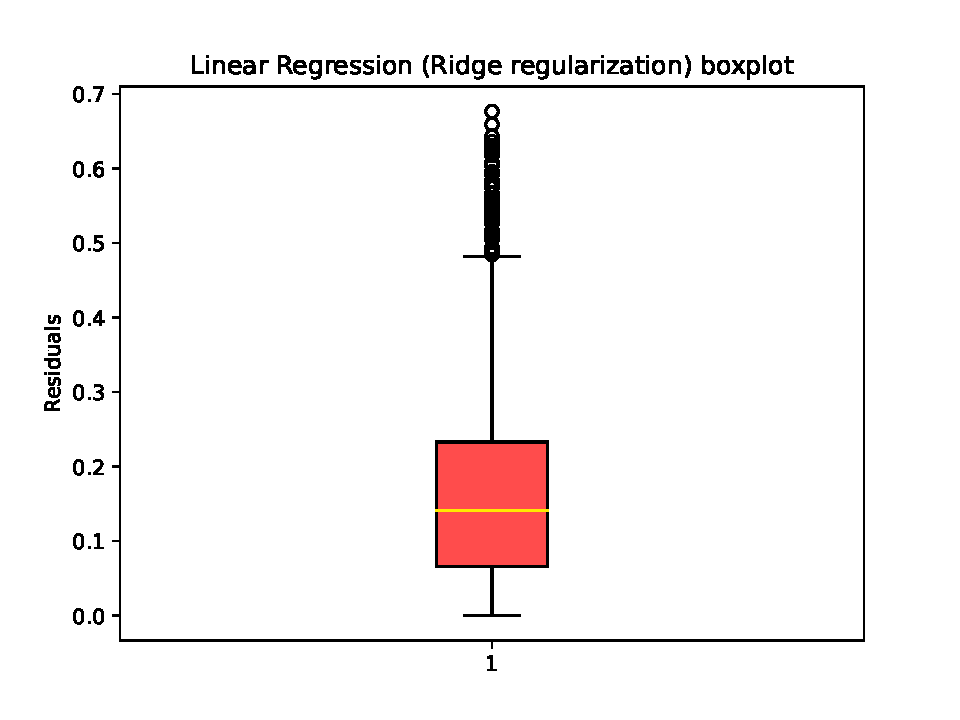
\includegraphics[scale=0.6]{hw03_plot_linreg_box} \par
  \vspace{-2mm}\hspace{-7.25mm}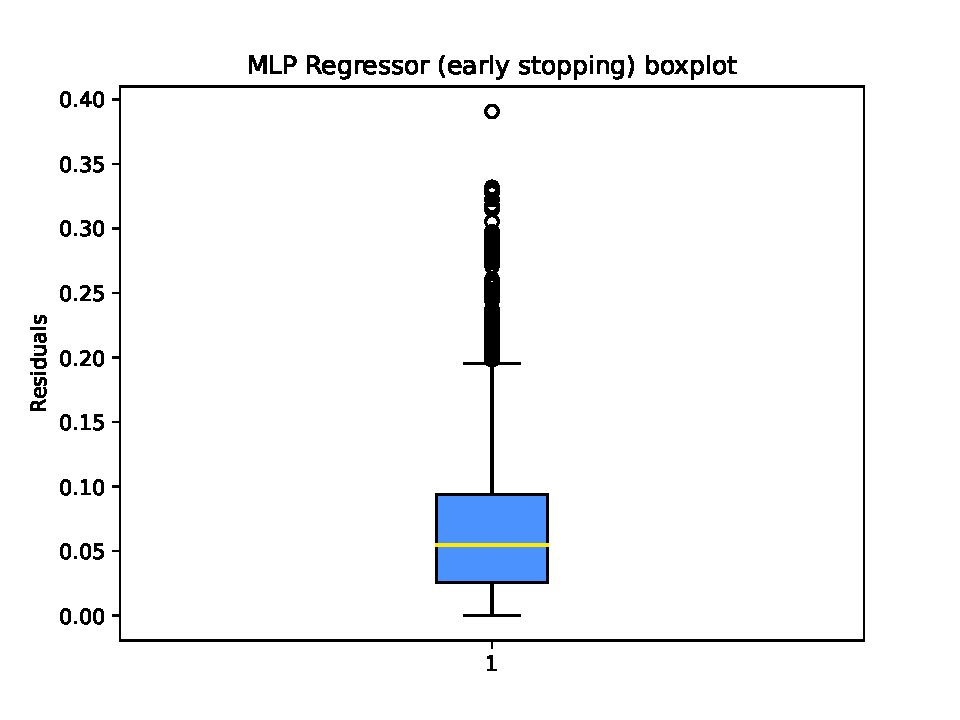
\includegraphics[scale=0.6]{hw03_plot_mlp1_box} \par
  &
  \hspace{-4.75mm}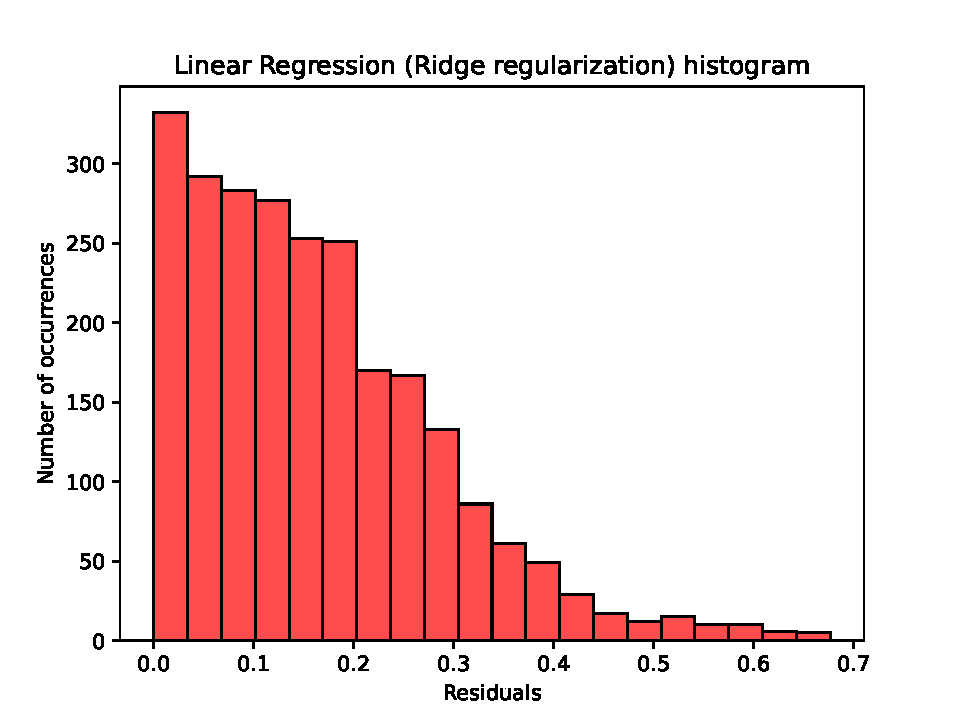
\includegraphics[scale=0.6]{hw03_plot_linreg_hist} \par
  \vspace{-2mm}\hspace{-4.75mm}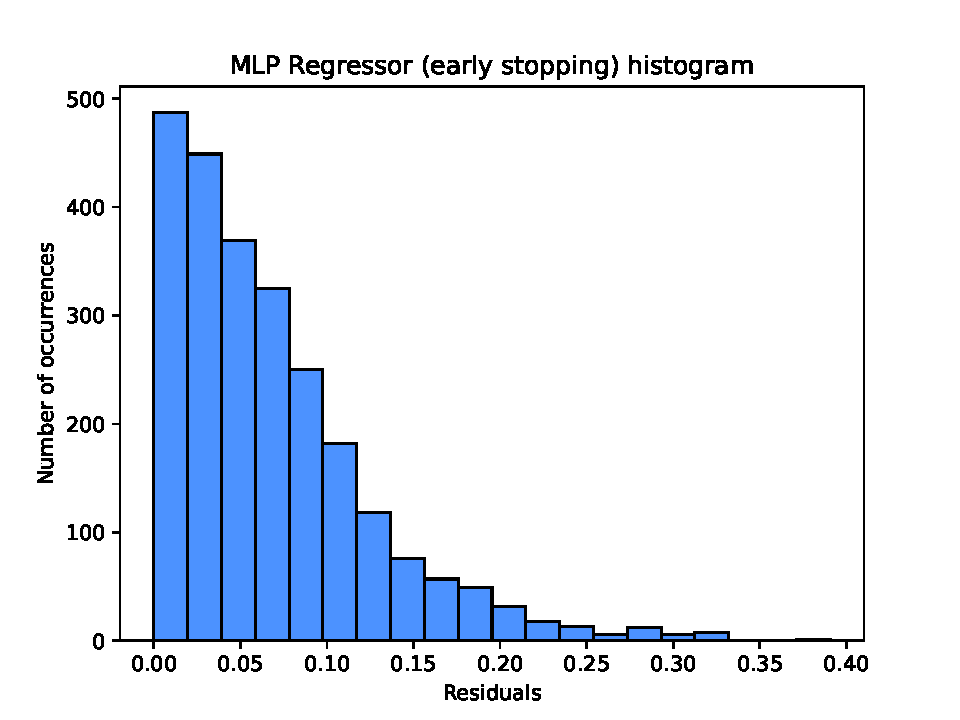
\includegraphics[scale=0.6]{hw03_plot_mlp1_hist} \par
\end{tabularx}
\end{flushleft}

\pagebreak
\hspace{-8.25mm}
\color{darkgray}
\renewcommand\tabularxcolumn[1]{m{#1}}
\begin{tabularx}{1.09\textwidth} {>{\raggedright\arraybackslash}X >{\centering\arraybackslash}X >{\raggedleft\arraybackslash}X}
  
\includegraphics[scale=0.2]{tecnico.pdf} &
  \textbf{Aprendizagem 2022/23} \par \textbf{Homework III - Group 66} &
  João Cardoso, 99251 \par José João Ferreira, 99259
\end{tabularx}
\renewcommand\tabularxcolumn[1]{p{#1}}
\color{black}

\begin{center}
\textbf{}
\end{center}

\begin{flushleft}
\vspace{-10mm}
\begin{tabularx}{1.09\textwidth} {X X}
    \vspace{-2mm}\hspace{-7.25mm}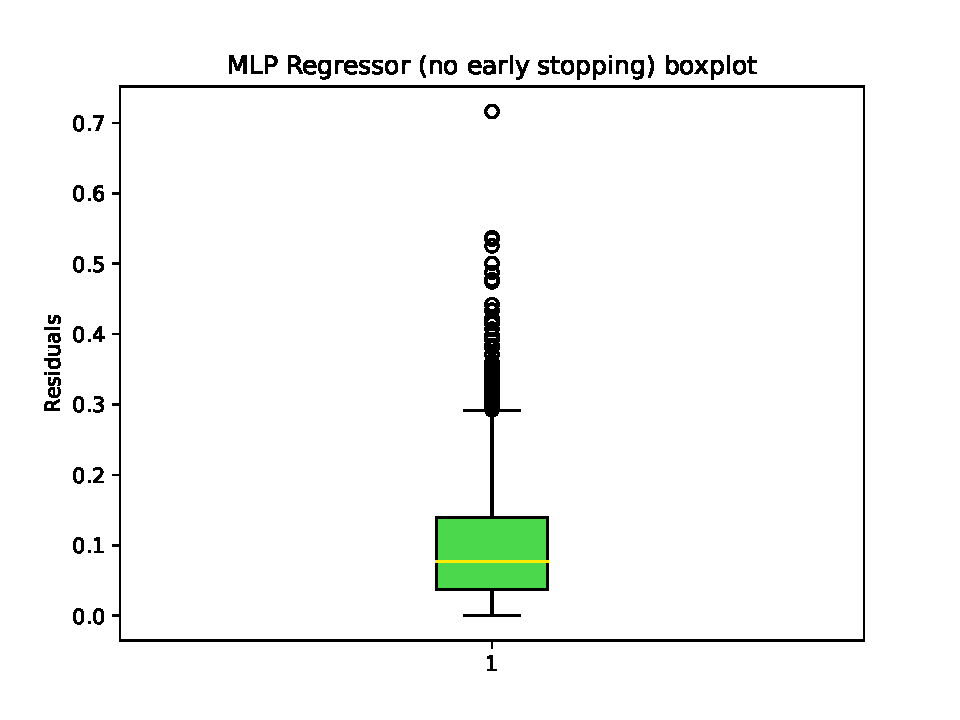
\includegraphics[scale=0.6]{hw03_plot_mlp2_box}
    &
    \vspace{-2mm}\hspace{-4.75mm}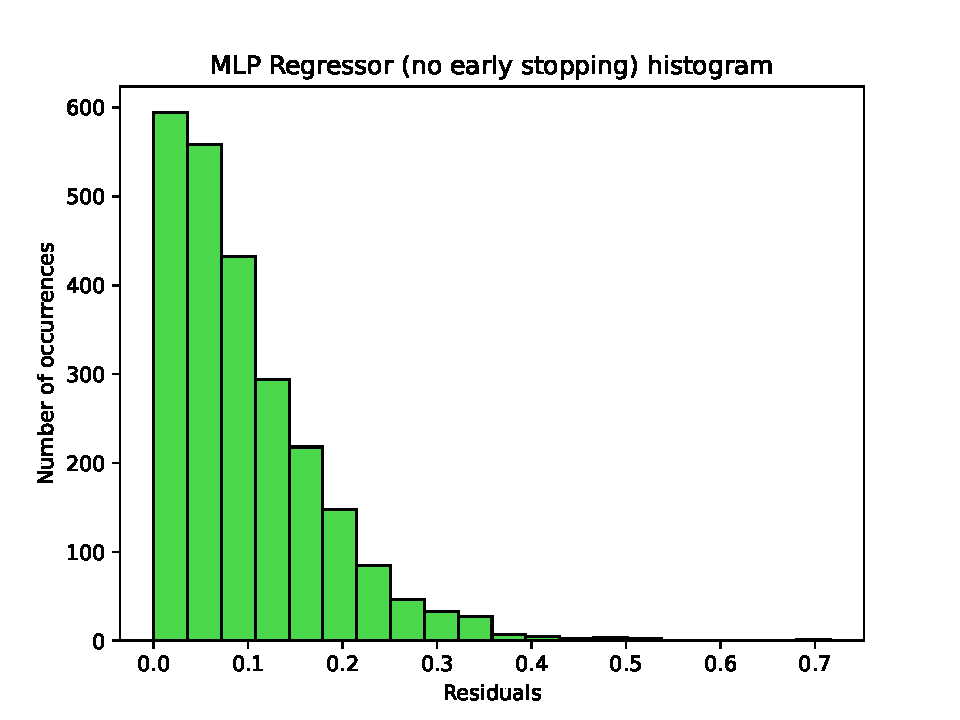
\includegraphics[scale=0.6]{hw03_plot_mlp2_hist} 
\end{tabularx}
\end{flushleft}

% PROBLEM 6
\begin{flushleft}
\vspace{-2mm}
\textbf{6)}
\end{flushleft}

% PROBLEM 7
\begin{flushleft}
\textbf{7)}
\end{flushleft}

\pagebreak
\hspace{-8.25mm}
\color{darkgray}
\renewcommand\tabularxcolumn[1]{m{#1}}
\begin{tabularx}{1.09\textwidth} {>{\raggedright\arraybackslash}X >{\centering\arraybackslash}X >{\raggedleft\arraybackslash}X}
  
\includegraphics[scale=0.2]{tecnico.pdf} &
  \textbf{Aprendizagem 2022/23} \par \textbf{Homework III - Group 66} &
  João Cardoso, 99251 \par José João Ferreira, 99259
\end{tabularx}
\renewcommand\tabularxcolumn[1]{p{#1}}
\color{black}

\begin{center}
\textbf{III. Appendix}
\end{center}

\definecolor{backcolour}{rgb}{0.95,0.95,0.92}
\definecolor{codegreen}{rgb}{0,0.6,0}
\definecolor{codepurple}{rgb}{0.58,0,0.82}
\definecolor{codegray}{rgb}{0.5,0.5,0.5}
\definecolor{codered}{rgb}{0.75,0.25,0}
\definecolor{codeyellow}{rgb}{0.55,0.55,0.0}
\definecolor{codeForestGreen}{rgb}{0.05,0.65,0.55}

\lstdefinestyle{mystyle}{
    backgroundcolor=\color{backcolour},
    commentstyle=\color{codegreen},
    keywordstyle=\color{codepurple},
    numberstyle=\tiny\color{codegray},
    stringstyle=\color{codered},
    emph=[0]{loadarff,train_test_split,mean_absolute_error,drop,print,format,abs,boxplot,title,ylabel,show,hist,xlabel},
    emphstyle=[0]\color{codeyellow},
    emph=[1]{pandas,pd,scipy,io,arff,sklearn,model_selection,linear_model,Ridge,neural_network,MLPRegressor,metrics,matplotlib,pyplot,DataFrame,range,dict},
    emphstyle=[1]\color{codeForestGreen},
    basicstyle=\ttfamily\footnotesize,
    breakatwhitespace=false,
    breaklines=true,
    captionpos=b,
    keepspaces=true,
    numbers=left,
    numbersep=7.5pt,
    showspaces=false,
    showstringspaces=false,
    showtabs=false,
    tabsize=2,
    language=Python,
    morekeywords={as}}
\lstset{style=mystyle}

\hspace{-8.25mm}
\begin{tabularx}{1.09\textwidth}{X}
  \lstinputlisting{hw03.py}
\end{tabularx}

\end{document}